\section{Accessing the Hardware}


\begin{figure}[H]
\centering
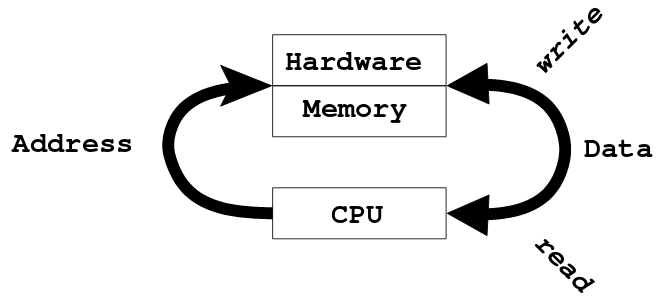
\includegraphics[width=0.6\textwidth]{figures/accessingHardware.png}
\caption{Access to the hardware}
\end{figure}

\textbf{Hardware looks like memory, but don't behaves like memory.}
The following two chapters describe the two possibilities to access the hardware (via pointers or then via extern).

\hypertarget{access-via-pointers}{%
\subsection{Access via pointers}\label{access-via-pointers}}

Following is described how the access to hardware works with pointers directly in the c file.

\begin{lstlisting}
volatile HWReg* const hwReg=(volatile HWReg* const) addr;
hwReg->someReg=someValue;
\end{lstlisting}

\hypertarget{access-via-extern}{%
\subsection{Access via extern}\label{access-via-extern}}

Following is described how the access to the hardware works with extern
management, like a linker script.

\begin{lstlisting}
// decleration
static volatile HWReg hwReg;
//access
hwReg.someReg=someValue;
\end{lstlisting}

\clearpage